\chapter{Numerical continuation} \label{sec: Continuation}

In order to find if a Hopf bifurcation occurs for the fixed tank pressure system, \cref{eq: QWFixedTankPressure}, a numerical continuation was performed using MatCont~\cite{Dhooge2003MATCONT}. This continuation would look for bifurcations of the unstable saddle at $(y_1,y_2,\tilde{B},\tilde{C})^T = (1,0,0,0)^T$. First, the pipe length parameter ($\gamma$) was varied while the other parameters are as in \cref{tab: ValveClosingQWMParameterValues}. However, convective effects and pipe friction were ignored ($\Lambda = \phi = 0$) and the tank was held at $p_0 = 1$. A Hopf bifurcation was found to occur at $\gamma \approx 0.85$.
%$\gamma = 0.850102$.
The Lyapunov coefficient of this bifurcation was calculated as  $5.4 \times 10^{-02}$, suggesting that a subcritical Hopf bifurcation occurs.

Once the subcritical Hopf bifurcation was found, the location at which the bifurcation occurs can be followed by varying two parameters. As the two parameters of interest, both the pipe length parameter, $\gamma$, and fixed tank pressure, $p_0$, were chosen. The numerical continuation then allows a two parameter bifurcation diagram
%, or alternatively a stability boundary,
to be created. \Cref{fig: BifurcationDiagram} shows these results.
% 
% Bifurcation diagram in $p_0$ and $\gamma$ space is
~
\begin{figure}[ht]
    \centering
    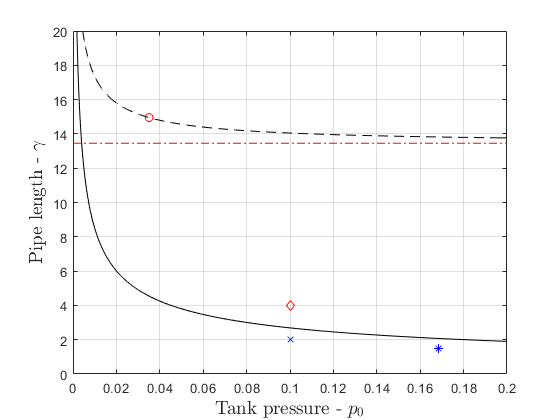
\includegraphics[width=0.7\textwidth]{Figures/BifurcationDiagram.png}
    \caption{Two parameter bifurcation diagram showing the numerical continuation of the subcritical Hopf bifurcation (lower solid black line). Also shown is the analytical stability boundary, calculated in \cref{subsec: QWMAnalyticalBound}, shown as the higher dashed black line. The critical pipe length $\gamma_c$ (\cref{eq: CritPipeLength}) is shown as a red dash-dotted horizontal line. Simulations performed in \cref{sec: QWSim} are denoted by the red circle, red diamond, blue cross, and blue asterisk (see \cref{sec: QWSim} for further details).}
    \label{fig: BifurcationDiagram}
\end{figure}
% 
% Parameters used are:
% ~
% \begin{equation*}
% \begin{split}
%     y_1 = 1 \, , \qquad
%     y_2 = 0 \, , \qquad
%     B = 0   \, , \qquad
%     C = 0
%     \\
%     \kappa = 0 \, , \qquad
%     \alpha = 8.5658 \, , \qquad
%     \delta = 1 \, , \qquad
%     \sigma = 10.3808 \, , \qquad
% \end{split}
% \end{equation*}

Also shown in \cref{fig: BifurcationDiagram} is the analytical stability boundary, calculated in \cref{subsec: QWMAnalyticalBound}, which tries to approximate where this Hopf bifurcation occurs. It is clear there is a large difference between these two results. However, as will be shown in \cref{sec: QWSim}, these two boundaries separate the dynamics into three %topologically equivalent
regions. For short pipe lengths, the Hopf bifurcation is yet to occur, and so any oscillations will decay. For longer pipe lengths, after the Hopf bifurcation occurs, oscillations will grow. However, these oscillations grow slower than the piston closes, and the closing dynamics dominates. This region could be considered where flutter would be observed. Finally, for very long pipe lengths, the oscillations grow faster than the main piston will close, meaning chatter will occur.

%% ADD SHORT SECTION EXPLAINING DIFFERENT TREND TO SPRING-OPERATED